
\subsection{\vectorsInSpaceTitle: Overview}

{\ttfamily
\fontdimen2\font=0.4em
\fontdimen3\font=0.2em
\fontdimen4\font=0.1em
\fontdimen7\font=0.1em
\hyphenchar\font=`\-

\hypertarget{scripts_vectors_in_space_n_vectors_overview}{What is the space} $\mathbb{R}^n$. In short it is the usual vectors we are used to. For example, if $n = 1$, then it is just the number line where we either move in the positive or negative directions, and we clearly have a notion of distance. This is something you should understand well, but ultimately there is nothing really interesting that goes on here.

Luckily when $n = 2$, things begin to get interesting. It is lucky for us because we can represent this by drawing arrows on paper. However what is interesting is that we no longer just have two directions, but an infinite number which we typically encapsulate as $0$ to $2\pi$ radians (i.e. 0 to 360 degrees). Recall that the length of the vector is also known as its magnitude. We can add vectors by putting them head to toe and we can scale our vectors, and this concept is useful in physics such as Force Vector Diagrams. So why is this system $\mathbb{R}^2$? The answer comes from trigonometry, and what I have described is polar coordinates which you should be able to translate back to the usual Cartesian coordinates of $(x, y)$. You still should be familiar with what things look like here.

Now for $\mathbb{R}^3$, if we look at this in Cartesian coordinates $(x, y, z)$, this is exactly the same as $\mathbb{R}^2$, just we can now move around in our usual ``3D'' space by basically being able to draw in the air. Now our notion of direction in somewhat more complicated using azimuth and altitude (see \hyperref[figure:azm_alt]{Figure~\ref*{figure:azm_alt}} below), but it is secretly still there. So we will just use the tuple to encapsulate the data of it's direction and magnitude. Also we can equivalently write our tuple $(x,y,z)$ as
\[
\begin{pmatrix}x \\ y \\ z \end{pmatrix}
\]
so our notation is consistent with matrix multiplication. Thus for all $n \geq 3$, we just use the tuple $(x^1, x^2, \dotsc, x^n)$ to encapsulate our direction and magnitude and you can just treat vectors in $\mathbb{R}^n$ the same way as you would for vectors in $\mathbb{R}^2$.

\begin{figure}
\label{figure:azm_alt}
\begin{center}
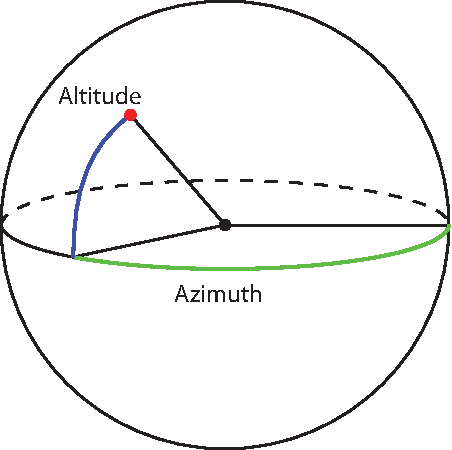
\includegraphics[scale=0.7]{\vectorsInSpacePath/azm_alt_diagram.pdf}
\end{center}
\caption{The azimuth and altitude in spherical coordinates.}
\end{figure}

Just one final closing remark; I have been somewhat sloppy through here on points and vectors, so make sure you read the note: \hyperlink{note_points_versus_vectors}{Points Versus Vectors} or \hyperref[points_vs_vectors]{Appendix~\ref*{points_vs_vectors}}.

} % Closing brace for the font

\newpage
